\documentclass{article}\usepackage{graphicx, color}
%% maxwidth is the original width if it is less than linewidth
%% otherwise use linewidth (to make sure the graphics do not exceed the margin)
\makeatletter
\def\maxwidth{ %
  \ifdim\Gin@nat@width>\linewidth
    \linewidth
  \else
    \Gin@nat@width
  \fi
}
\makeatother

\IfFileExists{upquote.sty}{\usepackage{upquote}}{}
\definecolor{fgcolor}{rgb}{0.2, 0.2, 0.2}
\newcommand{\hlnumber}[1]{\textcolor[rgb]{0,0,0}{#1}}%
\newcommand{\hlfunctioncall}[1]{\textcolor[rgb]{0.501960784313725,0,0.329411764705882}{\textbf{#1}}}%
\newcommand{\hlstring}[1]{\textcolor[rgb]{0.6,0.6,1}{#1}}%
\newcommand{\hlkeyword}[1]{\textcolor[rgb]{0,0,0}{\textbf{#1}}}%
\newcommand{\hlargument}[1]{\textcolor[rgb]{0.690196078431373,0.250980392156863,0.0196078431372549}{#1}}%
\newcommand{\hlcomment}[1]{\textcolor[rgb]{0.180392156862745,0.6,0.341176470588235}{#1}}%
\newcommand{\hlroxygencomment}[1]{\textcolor[rgb]{0.43921568627451,0.47843137254902,0.701960784313725}{#1}}%
\newcommand{\hlformalargs}[1]{\textcolor[rgb]{0.690196078431373,0.250980392156863,0.0196078431372549}{#1}}%
\newcommand{\hleqformalargs}[1]{\textcolor[rgb]{0.690196078431373,0.250980392156863,0.0196078431372549}{#1}}%
\newcommand{\hlassignement}[1]{\textcolor[rgb]{0,0,0}{\textbf{#1}}}%
\newcommand{\hlpackage}[1]{\textcolor[rgb]{0.588235294117647,0.709803921568627,0.145098039215686}{#1}}%
\newcommand{\hlslot}[1]{\textit{#1}}%
\newcommand{\hlsymbol}[1]{\textcolor[rgb]{0,0,0}{#1}}%
\newcommand{\hlprompt}[1]{\textcolor[rgb]{0.2,0.2,0.2}{#1}}%

\usepackage{framed}
\makeatletter
\newenvironment{kframe}{%
 \def\at@end@of@kframe{}%
 \ifinner\ifhmode%
  \def\at@end@of@kframe{\end{minipage}}%
  \begin{minipage}{\columnwidth}%
 \fi\fi%
 \def\FrameCommand##1{\hskip\@totalleftmargin \hskip-\fboxsep
 \colorbox{shadecolor}{##1}\hskip-\fboxsep
     % There is no \\@totalrightmargin, so:
     \hskip-\linewidth \hskip-\@totalleftmargin \hskip\columnwidth}%
 \MakeFramed {\advance\hsize-\width
   \@totalleftmargin\z@ \linewidth\hsize
   \@setminipage}}%
 {\par\unskip\endMakeFramed%
 \at@end@of@kframe}
\makeatother

\definecolor{shadecolor}{rgb}{.97, .97, .97}
\definecolor{messagecolor}{rgb}{0, 0, 0}
\definecolor{warningcolor}{rgb}{1, 0, 1}
\definecolor{errorcolor}{rgb}{1, 0, 0}
\newenvironment{knitrout}{}{} % an empty environment to be redefined in TeX

\usepackage{alltt}
\usepackage{spconf,amsmath,graphicx,color,hyperref}

\newcommand{\todo}[1]{\textcolor{red}{#1}}

\title{HIPPOCAMPAL SEGMENTATION WITH A VERY SMALL ATLAS LIBRARY: THE MAGET
BRAIN ALGORITHM} 
\name{  Jon Pipitone$^{1}$ Jason P. Lerch$^{4,5}$ Miriam Friedel$^{4,5}$
        Aristotle Voineskos$^{1,3}$ Mallar Chakravarty$^{1,2,3}$ }  

\address{
$^1$ Kimel Family Translational Imaging Genetics Research Laboratory, \\
     Research Imaging Centre, Centre for Addiction and Mental Health, Toronto, ON, Canada \\
$^2$ Institute of Biomaterials and Biomedical Engineering, University of
     Toronto, Toronto, ON, Canada \\
$^3$ Department of Psychiatry, University of Toronto, Toronto, ON, Canada \\
$^4$ Program in Neuroscience and Mental Health, The Hospital for Sick Children,
     Toronto, ON, Canada \\
$^5$ Department of Medical Biophysics, University of Toronto, Toronto, ON, Canada
}

\begin{document}

\maketitle       

\begin{abstract}
Neuroimaging research often relies on automated anatomical segmentations of MR
images of the brain. Current multi-atlas based approaches provide accurate
segmentations of brain images by propagating region labels from manual
delineations to unlabeled images. Unfortunately, these approaches often rely on
a large number of such manual-segmentated atlases which take time and
significant expertise to produce. We present an algorithm for the automatic
segmentation of the hippocampus that minimizes the number of atlases needed
whilst still achieving similar accuracy to  other multi-atlas approaches.  We
perform repeated random subsampling validation on the IBSR dataset to compare
our approach to multi-atlas segmentation using the full IBSR dataset, and to
single-atlas (model-based) segmentation. Our results show that with only 8
input atlas, MAGeT brain can achieve to within 2.0\% segmentation accuracy of
the multi-atlas approach using 17 input atlases (mean $\kappa = 0.775$ vs.
$\kappa = 0.791$).

\end{abstract}

\begin{keywords}
hippocampus, segmentation, multi-atlas, automated
\end{keywords}

\section{Introduction}
\label{sec:intro}

The hippocampus is of particular interest to many researchers because it is
implicated in forms of brain dysfunction such as Alzheimer's disease and
schizophrenia, and has functional significance in cognitive processes such as
learning and memory.  For many research questions involving magnetic resonance
imaging (MRI) data accurate identification of the hippocampus and its
subregions in participant MR images is a necessary first step to better
understand the individual neuroanatomy of specific subjects.  

Currently, the gold standard for neuroanatomical segmentation is manual
labelling by an expert human rater.  This is problematic for segmentation of
the hippocampus for several reasons.  First, manual segmentation takes a
significant investment of time and expertise \cite{Hammers2003} which may not
be readily available to researchers or clinicians.  Second, the amount of data
produced in neuroimaging experiments increasingly exceeds the capacity for
identification of specific neuroanatomical structures by an expert manual
rater.  Third, the true delination of hippocampal anatomy in MR images is
disputed\cite{Geuze2004}, as evidenced by efforts to create an unified
segmentation protocol\cite{Jack2011}.  Compounding each of these problems
is the significant neuroanatomical variability in the hippocampus
throughout the course of aging, development, and neuropsychiatric
disorders\cite{someone}.

As well, it may be necessary to use several different hippocampal
definitions or, in fact, make research-specific modifications in order to test
hypotheses (for example, \cite{Poppenk2011} found that overall hippocampal
volume difference did not predict recollection memory performance but by
dividing the hippocampus into anterior and posterior regions, a predictive
volume difference was found).  Thus, whilst manual segmentation of the
hippocampus is an important technique, it may be a bottleneck for researchers
or clinicians who do not have access to the needed human expertise.

Automated segmentation techniques attempt to overcome the need for human
expertise by performing segmentations computationally.  A popular class of
automated methods, {\it multi-atlas-based segmentation}, rely on a set of
expertly labeled neuroanatomical atlases. Each atlas is warped to fit a
subject's neuroanatomy using nonlinear registration
techniques\cite{Collins1995,Klein2009}.  Atlas labels are then transformed
by this warping and a {\it label fusion} technique, such as voxel-wise
voting, is used to merge the labellings from each atlas into a final
segmentation for a subject.  

Many descriptions of multi-atlas-based segmentation algorithms report relying on an
atlas library containing between 30 and 80 expertly labeled
brains\cite{Heckemann2011,Collins2010,Aljabar2009,Leung2010,Lotjonen2010}.
As noted, the production of an atlas library requires significant manual
effort, and is limited since the choice of atlases or segmentation protocol may
not reflect the underlying neuroanatomical variability of the population under
study or be suited to answer the research questions at hand.

In this paper we propose an automated segmentation technique to address the
above issues found in existing multi- atlas-based methods. Principly, our
method aims to dramatically reduce the number of manually labelled atlases
needed (under 10). It does this by using the small atlas library to boot-strap
a much larger "template library", which is then used to segment the subjects in
similar fashion as other multi-atlas-based methods. Our approach has the
additional advantage of using the unique subject population on hand to
initialise the segmentation analysis.

The essential insight of generating a template library is not new.  Heckemann
\cite{Heckemann2006} compared generating a template library from a single atlas
to standard multi-atlas segmentation and found poor performance and so deemed
the approach as inviable.  The LEAP algorithm \cite{Wolz2010} proceeds by
iteratively segmenting the unlabelled image most similar to the atlas library
images and then incorporating the now-labelled image into the atlas library,
but requires 30 starting atlases.  The novelty of our method is to demonstrate
the possibility of producing comparable segmentation accuracy to these and
other multi-atlas-based methods whilst using significantly fewer manually
created atlases.

In previous work from our group \cite{Chakravarty2011}, we applied MAGeT brain
to the segmentation the striatum, globus pallidus, and thalamus using a single
histologically-derived atlas. In the present work we extend our approach to the
hippocampus, a much more difficult structure to segment, and perform a thorough
validation over a range of atlas and template library sizes. Due to the small
number of atlases required, our method could easily accommodate different
hippocampal definitions. Our aim is not to improve on segmentation accuracy
beyond existing methods, but instead to provide a method that trades off manual
segmentation expertise for computational processing time whilst providing
sufficient accuracy for clinical and research applications.


\section{Materials and Methods} 
\subsection{The Multiple Automatically Generated Templates (MAGeT) Algorithm}

In this paper, we use the term {\it atlas} to mean any manually segmented MR
image, and the term {\it atlas library} to mean a set of such images.  We use
the term {\it template} to refer to any MR image, and associated labelling,
used to segment another image, and the term {\it template library} to refer to
a set of such images.  An atlas library may be used as a template library but,
as we will discuss, a template library may also be composed of images with
computer generated labellings. 

The segmentation approach we propose is best understood as an extension of
traditional multi-atlas segmentation.  In multi-atlas segmentation, an atlas
library and unlabelled MR images are given as input.  Every atlas image is
nonlinearly registered to each unlabelled image, and then each atlas' labels
are propagated via the resulting transformations.  These labels are then fused
to produce a single, definitive segmentation by some label fusion method (e.g.
voxel-wise majority vote). 

Our extension adds a preliminary stage in which a template library is
constructed from input images, and used in place of an atlas library in the
standard multi-atlas-based method.  To create the template library, labels from
each atlas image are propagated to each template library image via the
transformation resulting from a non-linear registration between pair of images.
As a result, each template library image has a label from each atlas.
Traditional multi-atlas segmentation is then used to produce segmentations for
the entire set of unlabelled images (including those images used in the
template library). 

Label fusion is performed by cross-correlation weighted voting, a strategy
weighted towards an optimal combination of subjects from the template library
which has been previously shown to improve segmentation
accuracy\cite{Aljabar2009,Collins2010}. In this method, each template library
image is ranked in similarity to each unlabelled image by the normalized
cross-correlation of image intensities after linear registration in a region of
interest (ROI) generously encompassing hippocampus.  Only the top n ranked
template library image labels are used in a voxel-wise majority vote. The ROI
is heuristically defined as the extent of all atlas labels after linear
registration to the template, dilated by three voxels\cite{Chakravarty2012}.

\subsection{MRI dataset evaluated}

For evaluation purposes we used the publicly available IBSR dataset.  This
dataset consists of T1 weighted MR image volumes from 18 subjects (4 females,
14 males) with ages between 7 and 71 years. Image dimensions for all MR volumes
are normalized to  $256  \times 256 \times 128$ voxels, with the voxel size
ranging from $0.8 \times 0.8 \times 1.5 mm$ to $1.0 \times 1.0 \times 1.5 mm$.
The images come 'positionally normalized' into the Talairach orientation
(rotation only), and processed by the CMA 'autoseg' biasfield correction
routines. The MR brain data sets and their manual segmentations are publicly
available and were provided by the Center for Morphometric Analysis at
Massachusetts General Hospital and are available at
\href{http://www.cma.mgh.harvard.edu/ibsr/}
{\nolinkurl{http://www.cma.mgh.harvard.edu/ibsr/}}. 

\subsection{Image Processing and Registration Method}
The N3 algorithm \cite{Sled1998} is first used to minimize the intensity
nonuniformity in each image.  Image registration is carried out in two phases.
In the first, a 12-parameter linear transformation (3 translations, rotations,
scales, shears) is estimated between images using an algorithm that maximizes
the correlation between blurred MR intensities and gradient magnitude over the
whole brain \cite{Collins}.  In the second phase, nonlinear registration is
completed using the ANIMAL algorithm \cite{Collins1995}: an iterative procedure
that estimates a 3D deformation field between two MR images. At first, large
deformations are estimated using blurred version of the input data. These
larger deformations are then input to subsequent steps where the fit is refined
by estimating smaller deformations on data blurred with a Gaussian kernel with
a smaller FWHM. The final transformation is a set of local translations defined
on a bed of equally spaced nodes that were estimated through the optimization
of the correlation coefficient. For the purposes of this work we used the
regularization parameters optimized in Robbins et al.\cite{Robbins2004}. It
should be noted that the MAGeT brain algorithm is not dependant on this, or
any, particular choice of registration method\cite{Chakravarty2011}.

\subsection{Experiments}

We explored how varying the size of the atlas library and the template library
effects labeling accuracy.  For each parameter setting we conducted 30 rounds
of random subsampling cross-validation using the 18 manual segmented templates
from the IBSR dataset as input. In each round, atlases were randomly chosen
from the IBSR dataset and the remaining images are used both as template
library images and unlabeled subjects to be labeled using the MAGeT brain
algorithm.  We varied the size of the atlas library from 3 to 8, and used
cross-correlation weighted label fusion to select the top $n$ candidate
templates from the remaining images.  $n$ was varied in the range $[3, 18-a]$,
where $a$ is the size of the atlas library.

\subsection{Evaluation}
\subsubsection{Goodness-of-fit}
Automatically produced segmentations are evaluated against IBSR manual
segmentations dataset using the Dice Kappa ($\kappa$) overlap metric, $\kappa =
{2a}/{(2a+b+c)}$, where $a$ is the number of voxels common to both
segmentations and $b+c$ is the sum of the voxels uniquely identified in either
segmentation.

\subsubsection{Comparison Approaches}
The resulting segmentations from each of our experiments are compared to those
produced from two alternative segmentation approaches. The {\it single-atlas}
approach uses one atlas to segment a unlabelled subject by directly propagating
labels from the atlas by way of nonlinear registration.  We computed a
single-atlas segmentation for each image in the IBSR dataset from each of the
other 17 labelled images.  Similarly, we computed a segmentation for each image
using the {\it multi-atlas} approach, described above, using the other 17
images as the atlas library.  Additionally, we also varied the number of atlas
images used in the label fusion step by employing cross-correlation weighted
voting.  In total we evaluated approximately $52,000$ segmentations for the
work presented in this manuscript.

\section{Results}

Sample segmentations from a single IBSR subject compared with the gold-standard
segmentation are in Fig.  \ref{montage}.  As the size of the template library
is increased, the number of false negatives in the hippocampal tail region is
reduced.  This is correlated with an increase in segmentation accuracy.

\begin{figure}[h]
\begin{minipage}[b]{1.0\linewidth}
  \centering
  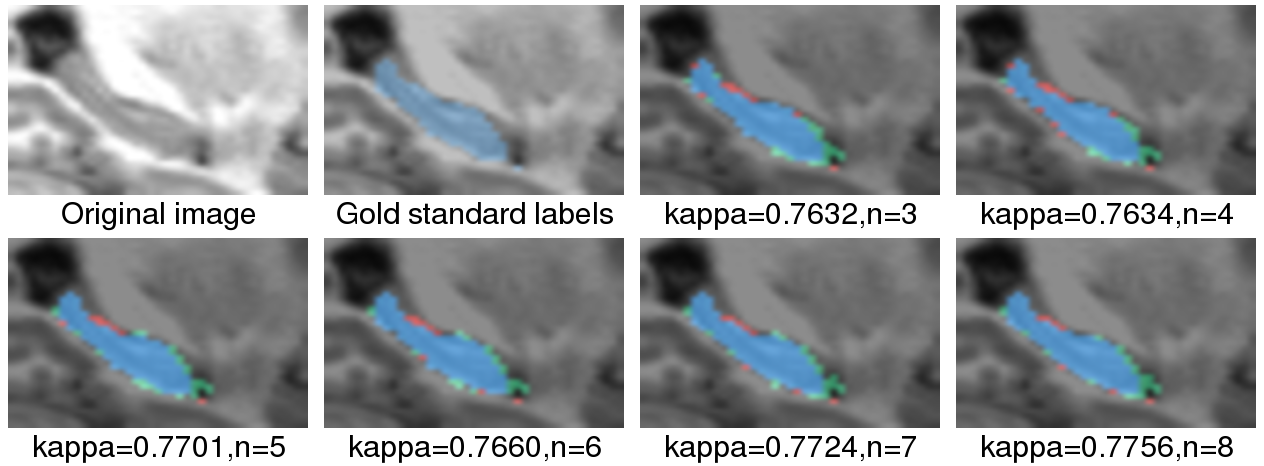
\includegraphics[width=\textwidth]{montage.png}
\end{minipage}
\caption{{\em Sample MAGeT brain segmentations.} 
Segmentations of a single subject are shown when three atlases are used, with
varying template library size $n$. Blue colouring represents agreement between
the gold-standard and MAGeT brain. Green colouring indicates false positive
voxels labelled by MAGeT brain, and red colouring indicates false negative
voxels.
} 
\label{montage}
\end{figure}

MAGeT brain shows distinct improvement in segmentation accuracy with increasing
atlas library size (Fig. \ref{results}), reaching its highest accuracy using 8
atlases (mean $\kappa = 0.775$).  This level of accuracy is within 2.0\% of the
multi-atlas approach (mean $\kappa = 0.791$) using 17 atlases. With only 3
atlases, MAGeT brain reaches to within 6.5\% accuracy of the multi-atlas
approach, and performs significantly better than the average single-atlas
performance. Surprisingly, our results do not show any significant improvements
in segmentation accuracy when applying cross-correlation weighted voting to
reduce the number of template labels being fused.

\begin{figure}
\begin{minipage}[b]{1.0\linewidth}
  \centering
  %\includegraphics[width=\textwidth]{results}
\begin{knitrout}
\definecolor{shadecolor}{rgb}{0.969, 0.969, 0.969}\color{fgcolor}\includegraphics[width=\maxwidth]{figure/unnamed-chunk-1} 
\end{knitrout}

\end{minipage}
\caption{
Mean performance of MAGeT brain with varying atlas library size and number of
template labels fused. Also shown is the mean multi-atlas performance when
using an atlas library of 17 images and varying the number of labels fused, as
well as the mean performance of single-atlas segmentations.  Data is fit with
LOESS local regression smoothing lines, and include a standard deviation
ribbon.
}
\label{results}
\end{figure}

\section{Discussion}

In this paper, we have demonstrated that accurate segmentations can be produced
by automatically deriving a template library from a small set of input atlases.
MAGeT brain segmentations were compared to both single-atlas segmentations and
multi-atlas segmentations with cross-correlation voting.  For the IBSR dataset,
on average MAGeT brain achieves within 2.0\% of the segmentation accuracy of
the multi-atlas approach but requires only 8 atlases as compared to using the
entire IBSR manually segmented library of 17 atlases.

L\"{o}tj\"{o}nen et al.\cite{Lotjonen2010} report a Kappa of 0.814 on
hippocampal segmentation in the IBSR dataset using a multi-atlas approach where
atlas selection is based on the similarity between atlas and unlabeled subject
after nonlinear registration, and using STAPLE\cite{Warfield2004} for label
fusion.  Discrepancies between our results and the above results may be due to
choice of registration algorithm, regularization parameters, or similarity
metric for label fusion.  Performance may also be affected by the variability
in the IBSR data set (as previously noted by \cite{Klein2009}).  Future work
from our group will attempt to address some of these issues.

\subsection{Acknowledgements}
Computations were performed on the gpc supercomputer at the SciNet HPC
Consortium\cite{Loken2010}. SciNet is funded by: the Canada Foundation for
Innovation under the auspices of Compute Canada; the Government of Ontario;
Ontario Research Fund - Research Excellence; and the University of Toronto.

\bibliographystyle{IEEEbib}
\bibliography{references}
\end{document}


